\documentclass[10pt]{beamer}
%souza naves, n 576
\usetheme[everytitleformat=regular]{metropolis}

% Língua e acentos
\usepackage[brazil]{babel}
\usepackage[utf8]{inputenc}
\usepackage[T1]{fontenc}

\usepackage{booktabs}
\usepackage[scale=2]{ccicons}

\usepackage{pgfplots}
\usepgfplotslibrary{dateplot}

\title{Cálculo do fluxo de potência em sistemas de distribuição de energia elétrica}
\subtitle{Com otimização por redução de barras}
\date{\today}
\author{David Maykon Krepsky Silva}
\institute{Departamento de Engenharia Elétrica}
\titlegraphic{
\includegraphics[height=1.cm]{img/logo}}

\usepackage{ragged2e}

\usepackage{pgf-pie}
\usetikzlibrary{ shadows }
\usepackage[authoryear]{natbib}

\usepackage{multirow}

\begin{document}

\maketitle

\begin{frame}
  \frametitle{Sumário}
  \setbeamertemplate{section in toc}[sections numbered]
  \tableofcontents[hideallsubsections]
\end{frame}

\section{Objetivos}
\begin{frame}{Objetivos do trabalho}
    Objetivos primários:
    \begin{itemize}
        \item Implementação dos métodos \textit{Soma de Correntes} e \textit{Soma de potências} para o cálculo do fluxo de potência.
        
        \item Comparação de desempenho entre os métodos.
        
        \item Desenvolvimento e implementação do algoritmo de otimização do fluxo de potência por redução de barras.
    \end{itemize}
    
    Objetivo secundário:
    \begin{itemize}
        \item Desenvolvimento de programa gráfico para análise de sistemas de distribuição utilizando os algoritmos acima citados.
    \end{itemize}
\end{frame}

\section{Metodologia}

\begin{frame}{Metodologia}
    
    \begin{itemize}
        \item Uso de linguagem de programação C++.
        
        \item Desenvolvimento com o \textit{framework} Qt.
        
        \item Validação dos resultados através da comparação com resultados de outro programa.
        
        \item Teste de performance dos algoritmos implementados, com e sem a otimização.
    \end{itemize}
\end{frame}

\section{Sistema elétrico brasileiro}

\begin{frame}[fragile]
  \frametitle{Consumo de energia elétrica no Brasil}
    \begin{itemize}
        \item Em julho de 2015, foram consumidos \alert{45.149 GWh} de energia elétrica no Brasil \cite{boletimMME}.
        
        \item As crises hídricas encarecem o custo da energia elétrica, pois estimulam o uso de combustíveis fósseis.
        
        \item De forma a compensar o custo extra das usinas termo-elétricas, foi instaurado em 2015 o Sistema de Bandeiras Tarifárias.
    \end{itemize}
\end{frame}

\begin{frame}[fragile]
    \frametitle{Perfil do consumo - julho/2015}
    \begin{figure}
        \centering
        \caption{Perfil de consumo de energia elétrica no Brasil, julho de 2015}
        \begin{tikzpicture}
            \pie [radius = 2, rotate = 90, color = {green, cyan, orange, black!20, violet, red}, explode = {0, 0, 0, 0, 0, 0.2}, style = drop shadow, text = pin]{22.4/Residêncial, 31.1/Industrial, 15.0/Comercial, 4.5/Rural, 8.4/Outros, 18.5/Perdas}    
        \end{tikzpicture}
        \\
        \small Fonte: Ministério de Minas e Energia \cite{boletimMME}.
        \label{fig:perfil}
        \end{figure}
\end{frame}

\begin{frame}[fragile]
  \frametitle{Ineficiência do sistema}
  \begin{itemize}
      \item Em alguns estados, como no Piauí, as perdas chegam a \alert{29\%} \cite{CostaNorte}.
      
      \item As perdas técnicas (como as perdas nos cabos e nos transformadores) chegam a 13\% \cite{CostaNorte}, sendo maior que as perdas totais em países como os EUA, a qual fica em torno de 6\% \cite{Queiroz}.
      
      \item O prejuízo é avaliado em bilhões de reais por ano.
      
      \item As maiores perdas técnicas se encontram no sistema de distribuição.
    \end{itemize}
\end{frame}

\section{O fluxo de potência}

\begin{frame}[fragile]
  \frametitle{O que é}
  \justify
     O fluxo de potência (ou fluxo de carga) é um problema matemático, composto por um conjunto de equações algébricas não lineares, que permite determinar os valores de tensão e potência, bem como as perdas, para um sistema elétrico de potência em regime permanente.

\end{frame}

\begin{frame}{Utilidade}
    \justify
    Provê uma visão detalhada das condições de operação do sistema, permitindo:
    
    \begin{itemize}
        \item análise de segurança da rede;
        
        \item o planejamento de redes de transmissão/distribuição mais eficientes;
        
        \item otimização dos sistemas em operação.
       \end{itemize}
\end{frame}

\begin{frame}{Características dos sistemas de potência}
    \begin{itemize}
        \item Composto por \emph{barras}, geradores, cargas, transformadores, reatores \textit{shunt}, capacitores \textit{shunt} e linhas de transmissão/distribuição.
        
        \item Barras são do tipo PV, PQ e V$\theta$.
        
        \item Barras são interligadas por linhas, as quais possuem perdas.
    \end{itemize}
\end{frame}

\begin{frame}{Solução do fluxo de potência}
    \justify
    Devido a natureza não linear do problema, são necessários métodos numéricos iterativos para a determinar uma aproximação das incógnitas nas equações do fluxo de potência.
\end{frame}


\begin{frame}{Métodos para cálculo do fluxo de potência}
    \justify
    Apesar dos métodos de Gauss-Seidel e Newton-Raphson (e seus derivados) serem amplamente utilizados para o calculo do fluxo de potência em sistemas de transmissão de energia elétrica, os mesmos apresentam problemas de convergência e desempenho quando aplicados em sistemas de distribuição \cite{Eminoglu, Alsaadi, Reddy, Yao}.
\end{frame}

\section{Métodos para redes de distribuição}

\begin{frame}{Redes de distribuição}
    Os métodos empregados na solução de redes de distribuição aproveitam a topologia radial \cite{Cespedes}, ou fracamente malhada \cite{ShirmohammadiMono, Shirmohammadi3F}, para resolver o problema do fluxo de potência.
\end{frame}

\begin{frame}{Redes radiais}
\begin{figure}[H]
   \centering
   \caption{Sistema radial.}
   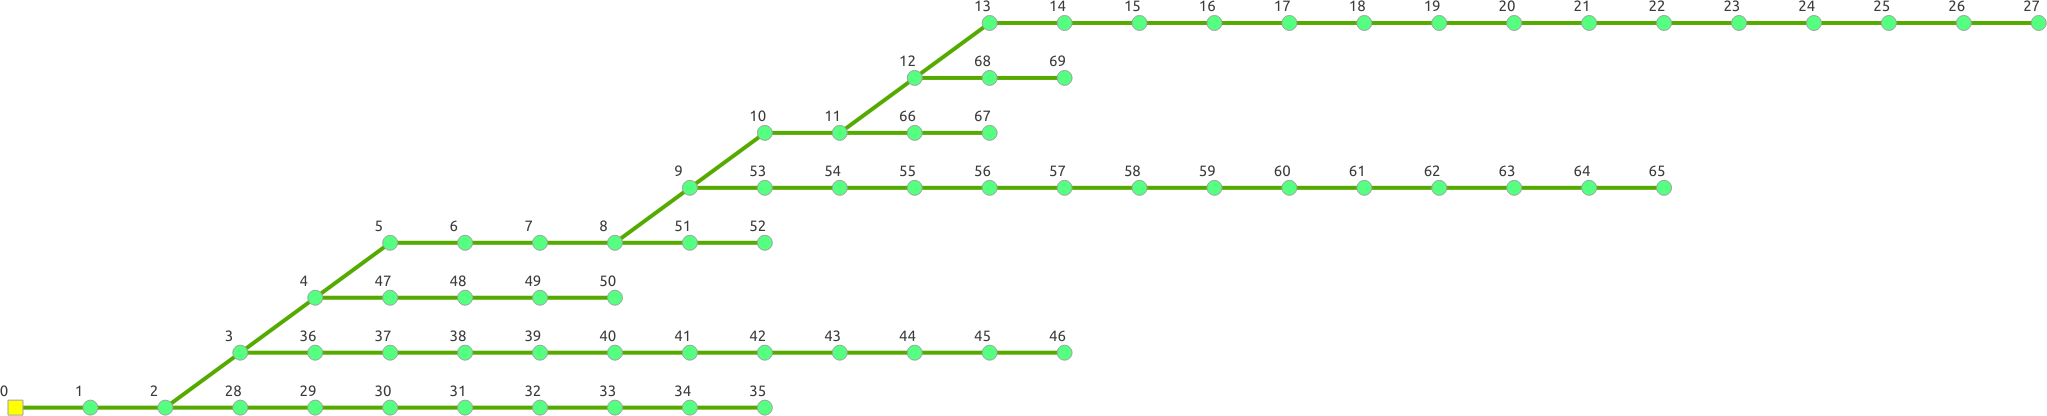
\includegraphics[scale=0.2]{img/69b}
   \label{fig:69b}
\end{figure}
\end{frame}

\begin{frame}{Redes malhadas}
    \begin{figure}[H]
        \centering
        \caption{Sistema malhado.}
        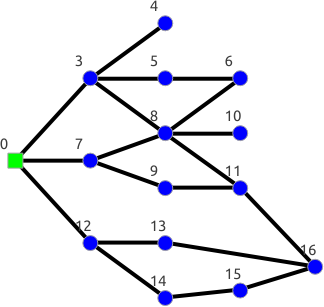
\includegraphics[scale=0.6]{img/malhado}
        \label{fig:malhado}
    \end{figure}
\end{frame}

\begin{frame}{Método Soma de Potências}
    Este método, proposto em \citep{Cespedes}, consiste em duas operações, uma a montante e outra a jusante. 
    
    \begin{itemize}
        \item Operação a montante: partindo dos nós finais até o nó inicial, são calculadas as potências equivalentes em cada nó (i.e., somando todas as potências que são alimentadas por cada nó e as suas perdas).
        
        \item Operação a jusante: dado que a tensão da barra de referência é conhecida, é aplicada a equação \ref{equ:cespedes} para o cálculo da tensão nas barras subsequentes.
        
        \item O critério de parada é determinado pela variação das perdas totais do sistema (equação \ref{equ:cespedesL}).
    \end{itemize}
\end{frame}

\begin{frame}{Método Soma de Potências}
    Equação para o cálculo das tensões:
    \begin{equation}
    \label{equ:cespedes}
    V_r^4 + [2 \cdot (PR+QX) -V_s^2] \cdot V_r^2 + (P^2 + Q^2) \cdot (R^2 + X^2) = 0.
    \end{equation}
    
    Perdas nas linhas:
    \begin{eqnarray}
    \label{equ:cespedesL}
    L_p = R \frac{(P^2 + Q^2)}{V_r^2} \\
    L_q = X \frac{(P^2 + Q^2)}{V_r^2}
    \end{eqnarray}
    Onde:
    \begin{itemize}
        \item \emph{s} é o nó fonte e \emph{r} é o nó à jusante;
        \item \emph{$V_s$} é o módulo da tensão em \emph{s};
        \item \emph{$V_r$} é o módulo da tensão em \emph{r};
        \item \emph{P} e \emph{Q} são as potências ativa e reativa equivalentes da carga;
        \item \emph{R} é a resistência e \emph{X} a reatância da linha de transmissão;
        \item \emph{$L_p$} e \emph{$L_q$} são as perdas ativas e reativas, respectivamente.
    \end{itemize}
    
\end{frame}

\begin{frame}{Desvantagens}
Desvantagens:
    \begin{itemize}
        \item Não calcula o ângulo das tensões.
        \item Aplicável somente a sistemas radiais.
    \end{itemize}
\end{frame}

\begin{frame}{Método Soma de Correntes}
    Proposto em \cite{ShirmohammadiMono, Shirmohammadi3F}, também consiste em duas operações, chamadas de varredura para trás (\textit{backward sweep}) e varredura para frente (\textit{forward sweep}). 
    
    \begin{itemize}
        \item Varredura para trás: assumindo um perfil de tensão inicial para as barras, o algoritmo começa calculando as correntes nos nós das camadas finais com a equação \ref{equ:shirmI}. Em seguida, é calculado a corrente da camada anterior, sendo que, a corrente nas barras dessa camada é a soma das correntes que vão e direção a camada seguinte (equação \ref{equ:shirmJ}).
        
        \item Varredura para frente: Ao chegar na barra de referência (a qual possui tensão e fase conhecidas), o algoritmo calcula a tensão nas barras subsequentes, considerando as correntes previamente calculadas e a queda de tensão nas linhas de distribuição, com a equação \ref{equ:shirmV}.
        
        \item O critério de parada é determinado pela variação da potência no sistema.
    \end{itemize}
\end{frame}

\begin{frame}{Equações do método Soma de Correntes}
   Corrente nas barras:
    \begin{equation}
    \label{equ:shirmI}
      \left[ \begin{matrix}
      I_{ia} \\
      I_{ib} \\
      I_{ic} \\
      \end{matrix} \right]  = 
      \left[ \begin{matrix}
      \left(S_{ia} \big / V_{ia}^{(k-1)} \right)^* \\
      \left(S_{ib} \big / V_{ib}^{(k-1)} \right)^* \\
      \left(S_{ic} \big / V_{ic}^{(k-1)} \right)^* \\
      \end{matrix} \right] -
      \left[ \begin{matrix}
      Y_{ia}^* & & \\
      & Y_{ib}^* & \\
      & & Y_{ic}^* \\
      \end{matrix} \right]
      \left[ \begin{matrix}
      V_{ia} \\
      V_{ib} \\
      V_{ic} \\
      \end{matrix} \right]^{(k-1)}
    \end{equation}
 
    Corrente nas linhas:
    \begin{equation}
    \label{equ:shirmJ}
     \left[ \begin{matrix}
     J_{la} \\
     J_{lb} \\
     J_{lc} \\
     \end{matrix} \right]^{(k)}  = -
      \left[ \begin{matrix}
      I_{ja} \\
      I_{jb} \\
      I_{jc} \\
      \end{matrix} \right]^{(k)} + \sum_{m \, \in \, M}
       \left[ \begin{matrix}
       J_{ma} \\
       J_{mb} \\
       J_{mc} \\
       \end{matrix} \right]^{k}
    \end{equation}
    
        Tensão nas barras:
        \begin{equation}
        \label{equ:shirmV}
        \left[ \begin{matrix}
        V_{ja} \\
        V_{jb} \\
        V_{jc} \\
        \end{matrix} \right]^{(k)}  =
        \left[ \begin{matrix}
        V_{ia} \\
        V_{ib} \\
        V_{ic} \\
        \end{matrix} \right]^{(k)} -
        \left[ \begin{matrix}
        Z_{aa,l} & Z_{ab,l} &  Z_{ac,l} \\
        Z_{ba,l} & Z_{bb,l} &  Z_{bc,l} \\
        Z_{ca,l} & Z_{cb,l} &  Z_{cc,l} \\
        \end{matrix} \right]
        \left[ \begin{matrix}
        J_{la} \\
        J_{lb} \\
        J_{lc} \\
        \end{matrix} \right]^{(k)}
        \end{equation}
\end{frame}

\begin{frame}{Equações do método Soma de Correntes}
 Onde:
 
    \begin{itemize}
    \item $I_{ia}, I_{ib}, I_{ic}$ são as injeções de corrente na barra \emph{i}.
    
    \item $S_{ia}, S_{ib}, S_{ic}$ são as injeções de potência programadas na barra \emph{i}.
    
    \item $V_{ia}, V_{ib}, V_{ic}$ são as tensões na barra \emph{i}.
    
    \item $Y_{ia}, Y_{ib}, Y_{ic}$ são as admitâncias dos elementos \textit{shunt} na barra \emph{i}.
    
    \item $J_{la}, J_{lb}, J_{lc}$ são as correntes na linha \emph{l}.
    
    \item \emph{k} é a iteração.
    \end{itemize}
    
    
\end{frame}

\begin{frame}{Otimização por redução de barras}
    Em andamento...
\end{frame}

\section{Resultados}

\begin{frame}{Validação dos algoritmos - Tensão}
    \begin{table}
        \caption{Tesões no sistema de 69 barras\footnote{Margem de erro 1\%}. Valores em volts.}
        \begin{tabular}{cccc}
            \toprule
            Barra & Soma de potências & Soma de correntes & Diferença \\
            \midrule
            0 & 12.661,3 & 12.661,3 & 0.00 \\
            1 & 12.660,9 & 12.660,9 & 0.00 \\
            2 & 12.660,4 & 12.660,4 & 0.00 \\
            3 & 12.660,4 & 12.660,4 & 0.00 \\
            4 & 12.659,2 & 12.659,2 & 0.00 \\
            5 & 12.648,8 & 12.648,8 & 0.00 \\
            6 & 12.535,7 & 12.535,7 & 0.00 \\
            7 & 12.418,1 & 12.418,1 & 0.00 \\
            8 & 12.390,0 & 12.390,0 & 0.00 \\
            9 & 12.375,7 & 12.375,7 & 0.00 \\
            \bottomrule
        \end{tabular}
    \end{table}
    
\end{frame}

\begin{frame}{Validação dos algoritmos - Perdas}
    \begin{table}
        \caption{Perdas no sistema de 69 barras\footnote{Margem de erro 1\%}. Valores em VA.}
        \begin{tabular}{ccccc}
            \toprule
            Nó inicial & Nó final & Soma de potências & Soma de correntes\\
            \midrule
            0 & 1 & 0.07498 + 0.17995j & 0.07498 + 0.17995j \\
            1 & 2 & 0.07498 + 0.17995j & 0.07498 + 0.17995j \\
            2 & 3 & 0.01431 + 0.01431j & 0.01431 + 0.01431j \\
            3 & 4 & 0.19493 + 0.46785j & 0.19493 + 0.46785j \\
            4 & 5 & 1.93656 + 2.26832j & 1.93656 + 2.26832j \\
            5 & 6 & 28.2383 + 14.3815j & 28.2383 + 14.3815j \\
            6 & 7 & 29.3461 + 14.9464j & 29.3461 + 14.9464j \\
            7 & 8 & 6.89402 + 3.51431j & 6.89402 + 3.51431j \\
            8 & 9 & 3.37479 + 1.71820j & 3.37479 + 1.71820j \\
            9 & 10 & 4.77740 + 1.57905j & 4.77740 + 1.57905j \\
            \bottomrule
        \end{tabular}
    \end{table}
\end{frame}

\begin{frame}{Comparação de desempenho sem otimização - Tempo}
    \begin{figure}
        \centering
        \caption{Tempo de convergência para os sistemas de teste.}
        \begin{tikzpicture}
        \begin{axis}[
        legend pos=north west,
        xlabel={Barras},
        ylabel={Duração [ms]},
        width=0.9\textwidth,
        height=6cm,
        ]
        
        \addplot plot coordinates {(14, 0) (69, 3) (136, 7) (794, 43) (3375, 204)};
        \addplot plot coordinates {(14, 0) (69, 2) (136, 4) (794, 65) (3375, 605)};
        
        \legend{Soma das potências, Soma das correntes}
        
        \end{axis}
        \end{tikzpicture}
    \end{figure}
\end{frame}

\begin{frame}{Comparação de desempenho sem otimização - Iterações}
    \begin{figure}
        \centering
        \caption{Número de iterações necessárias para convergência dos sistemas de teste.}
        \begin{tikzpicture}
        \begin{axis}[
        legend pos=north east,
        xlabel={Barras},
        ylabel={Número de iterações},
        width=0.9\textwidth,
        height=6cm,
        ]
        
        \addplot plot coordinates {(14, 5) (69, 7) (136, 6) (794, 6) (3375, 7)};
        \addplot plot coordinates {(14, 7) (69, 8) (136, 8) (794, 7) (3375, 7)};
        
        \legend{Soma das potências, Soma das correntes}
        
        \end{axis}
        \end{tikzpicture}
    \end{figure}
\end{frame}

\begin{frame}{Comparação de desempenho - com otimização}
    Necessário implementar o algoritmo de otimização.
\end{frame}

\begin{frame}{\textit{QuickFlow}}
    \begin{figure}[H]
        \centering
        \caption{Programa \textit{QuickFlow} para projeto e análise de sistemas de distribuição de energia elétrica.}
        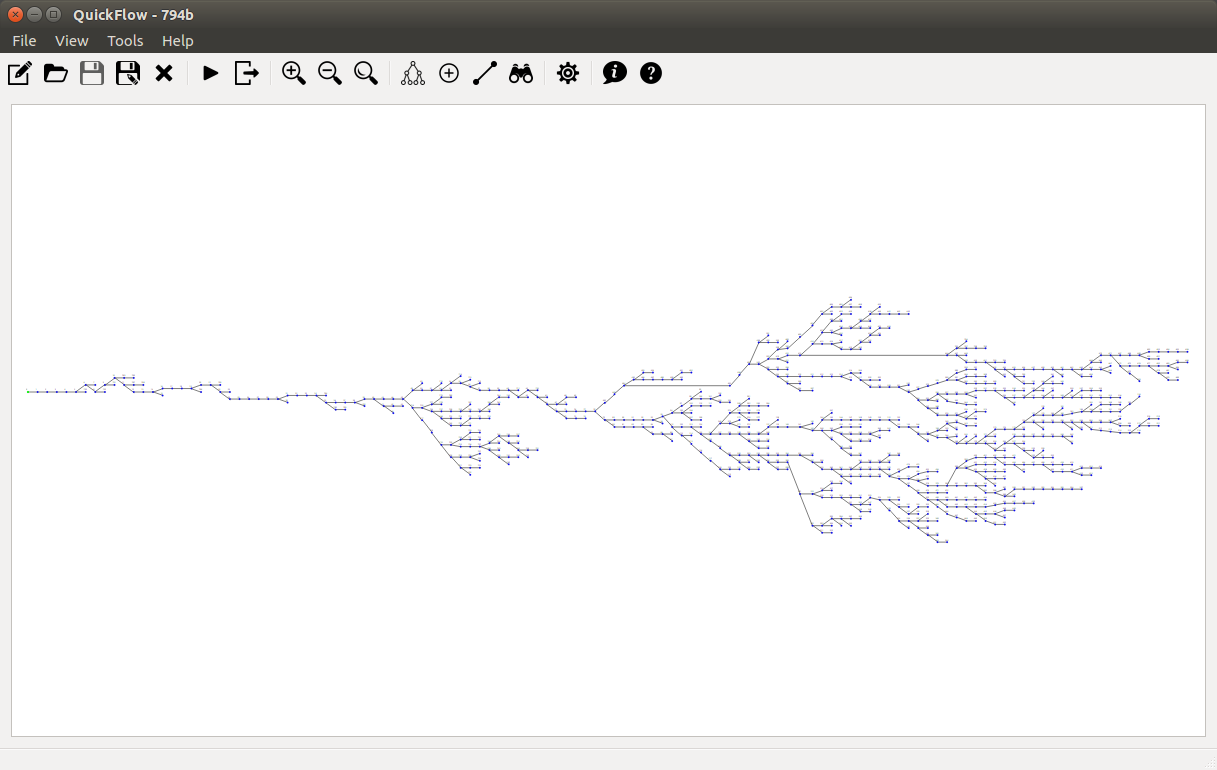
\includegraphics[scale=0.22]{img/quickflow}
        \label{fig:quickflow}
    \end{figure}
\end{frame}

\begin{frame}{\textit{QuickFlow}}
    \begin{figure}[H]
        \begin{itemize}
            \item Permite a criação, importação e modificação de sistemas de distribuição energia elétrica trifásicos.
            
            \item Possibilita o trabalho com várias unidades (metro, kilometro, pés, milhas e etc.).
             
            \item Permite trabalhar com múltiplos alimentadores.
             
            \item Realiza o cálculo do fluxo de potência utilizando os dois métodos citados anteriormente.
            
            \item Aplica a otimização por redução de barras para agilizar os cálculos (em desenvolvimento).
            
            \item Possui código fonte aberto. Está disponível em \href{http://www.github.com/DKrepsky/QuickFlow}{GitHub/QuickFlow}.
            
        \end{itemize}
    \end{figure}
\end{frame}

\begin{frame}{Conclusão}
    Até o presente momento, foi observado que os métodos de resolução do fluxo de potência, empregados no trabalho, se mostram bastante robustos em relação à convergência. O desempenho dos mesmos é satisfatório, sendo necessário poucos milissegundos, em um computador de uso pessoal, para o cálculo dos parâmetros em sistemas compostos por milhares de barras. Em relação a comparação entre os métodos, foi possível observar um melhor desempenho do método da soma das potências, porém, o mesmo não provê a informação sobre a fase das tensões na rede.
    Quanto a \textit{interface} gráfica, a mesma se mostrou bastante útil na análise de sistemas de distribuição de energia elétrica, agilizando a avaliação dos resultados e o teste com sistemas diferentes.
\end{frame}

\begin{frame}{Considerações finais}
    O trabalho desenvolvido é um passo inicial no desenvolvimento de uma ferramenta para análise do fluxo de potência. Assim, há a possibilidade de explorar uma grande quantidade de outros algoritmos, tanto de cálculo, como de formas de otimização para o fluxo de potência.
    Uma outra possibilidade é a integração de métodos para o calculo do fluxo de potência ótimo, o qual encontra o melhor estado de operação da rede, de modo a minimizar o custo do kilowatt hora entregue ao consumidor final.
\end{frame}

\begin{frame}[allowframebreaks]

  \frametitle{Referências}

  \bibliography{referencias}
  \bibliographystyle{plain}

\end{frame}

\plain{Perguntas?}

\end{document}
